% !TeX spellcheck = si_SI
\chapter{Teoretične osnove in pregled literature}\label{cha:teoreticne_osnove}

\section{Vsebina}\label{sec:vsebina}
Ne glede na to ali je naloga teoretično ali eksperimentalno usmerjena, je potrebno najprej obdelati teoretične osnove obravnavane tematike.

\subsection{Vir informacij}\label{sec:vir_informacij}
Pri pregledu literature naj bodo knjige in predvsem strokovni ter znanstveni članki glavni vir informacij. Pri spletnem iskanju člankov in ostale literature priporočamo uporabo naslednjih iskalnikov: Dikul, Web of Science, ScienceDirect in Google Scholar.

Več o citiranju virov si preberite v nadaljevanju te predloge.

\section{Podpoglavja in slogi}\label{sec:podpoglavja}
Posamezne dele smiselno razdelite v podpoglavja, ki naj bodo zaporedno oštevilčena. Oblika in slog naslovov naj ustreza tem, ki so prikazani v tej predlogi. Številčenje naj bo samodejno, tako kot je prikazano v tej predlogi. To predlogo neposredno uporabite za pisanje zaključnega dela, saj so vsi slogi že prednastavljeni (navaden slog, slog za poglavja in podpoglavja, slog za naslove preglednic in slik itn.).

\subsection{Podpoglavje 2. ravni}\label{sec:poglavje_2}
\subsubsection{Podpoglavje 3. ravni}\label{sec:poglavje_3}

Prve vrstice odstavkov naj ne bodo zamaknjene, naj pa bo med posameznimi odstavki po ena prazna vrstica. Med naslovom podpoglavja in koncem predhodnega besedila naj bosta 2 prazni vrstici razmika. Če se naslov podpoglavja začne takoj za naslovom podpoglavja višje ravni, naj med naslovoma ne bo praznih vrstic. Uporabite lahko največ 4 ravni naslovov, torej glavni naslov ter 3 ravni podnaslovov.

\textbf{Dodatna razmejitev besedila}\\
Če želite v zadnji, 4. ravni podpoglavja še dodatno ločiti posamezne dele besedila, lahko uporabite eno vrstico krepkega tiska \verb|\textbf{<>}|.

\subsubsection{Uporaba krepkega, poševnega in podčrtanega tiska}\label{sec:emphasis_types}

Poleg predhodnega primera je uporaba \textbf{krepkega tiska} smiselna:
\begin{itemize}
\item kadar v besedilu prvič omenimo in opredelimo zelo pomemben pojem za razumevanje naloge,
\item kadar želimo posebej poudariti kakšen del ali misel,
\item kadar želimo npr. pri naštevanju vidno ločiti posamezne dele besedila.
\end{itemize}

Kadar v besedilu uporabljamo besede iz tujih jezikov, uporabljamo poševni oz. kurzivni tisk (ang. \emph{italics}). \underline{Podčrtanega tiska} praviloma ne uporabljamo.


\subsubsection{Ravni naštevanja}\label{sec:itemizing}

Ne glede na to, koliko hierarhičnih ravni alinej je v besedilu uporabljenih za naštevanje (običajno ne več kot 2), v celotnem besedilu vedno uporabljamo enako kombinacijo ter način označevanja posameznih ravni alinej. S tem dosežemo poenoten videz besedila.

Za označevanje vseh ravni alinej uporabimo znak »--«. Urejanje odmikov od roba strani za posamezen nivo prepustimo \LaTeX u. Primer je prikazan v nadaljevanju:
\begin{itemize}
\item primer 1. ravni:
\begin{itemize}
\item primer 2. ravni,
\item primer 2. ravni,
\end{itemize}
\item primer 1. ravni:
\begin{itemize}
\item primer 2. ravni,
\item primer 2. ravni.
\end{itemize}
\end{itemize}

Pred novim odstavkom besedila naj bo za zadnjo alinejo 1 prazna vrstica presledka, oz. 2 prazni vrstici presledka, če zadnji alineji sledi naslov novega poglavja.

\section{Preglednice}\label{sec:preglednice}

Preglednice naj bodo zaporedno oštevilčene, za kar samodejno poskrbi \LaTeX. Preglednica naj bo sredinsko poravnana. Primer je prikazan v preglednici \ref{tab:ucinkovitost_procesov}.

Naslov preglednice z zaporedno številko preglednice in kratkim opisom naj bo nad preglednico. Kratek opis preglednice naj se začne z veliko začetnico in zaključi s končnim ločilom. Med besedilom in naslovom preglednice naj bo 1 (prazna) vrstica presledka, kot na primer pri preglednici \ref{tab:ucinkovitost_procesov}, razen če je naslov preglednice povsem na vrhu strani. Med preglednico in nadaljevanjem besedila naj bosta 2 prazni vrstici.

\begin{table}[ht!]
\caption{Učinkovitost procesov odstranjevanja različnih o\-nes\-na\-že\-val\-cev vode.} \label{tab:ucinkovitost_procesov}
\centering
\begin{tabular}{|l|@{}c|@{}c|@{}c|@{}c@{}|}
\hline
\multirow{4}*{\minitab[c]{Proces}} &
\multirow{4}*{\minitab[c]{Odstranitev\\mikro-\\organizmov}} &
\multirow{4}*{\minitab[c]{Odstranitev\\suspendiranih\\snovi}}&
\multirow{4}*{\minitab[c]{Odstranitev\\raztopljenih\\anorganskih\\snovi}}&
\multirow{4}*{\minitab[c]{Odstranitev\\raztopljenih\\organskih\\snovi}}\\
&&&&\\
&&&&\\
&&&&\\
\hline
\textbf{Biološki}&&&&\\
\hline
\quad Aktivno &
\multirow{2}*{\minitab[c]{+}} &
\multirow{2}*{\minitab[c]{+}} &
\multirow{2}*{\minitab[c]{-}} &
\multirow{2}*{\minitab[c]{+}}\\
\quad blato & & & &\\
\hline
\quad Anaerobna &
\multirow{2}*{\minitab[c]{-}} &
\multirow{2}*{\minitab[c]{+}} &
\multirow{2}*{\minitab[c]{-}} &
\multirow{2}*{\minitab[c]{+}}\\
\quad obdelava & & & &\\
\hline
\quad Biofiltri & - & - & - & +\\
\hline
\textbf{Kemični}&&&&\\
\hline
\quad Kloriranje & + & + & - & +\\
\hline
\quad Ozoniranje & + & + & - & $\circ$\\
\hline
\quad Koagulacija & + & + & - & +\\
\hline
\textbf{Fizikalni}&&&&\\
\hline
\quad Adsorpcija &
\multirow{2}*{\minitab[c]{}} &
\multirow{2}*{\minitab[c]{}} &
\multirow{2}*{\minitab[c]{}} &
\multirow{2}*{\minitab[c]{}}\\
\quad na aktiv. oglju:& & & &\\
\hline
\quad \quad v granulah	& - & + & - & +\\
\hline
\quad \quad v prahu & + & + & - & +\\
\hline
\quad Konvencionalna &
\multirow{2}*{\minitab[c]{-}} &
\multirow{2}*{\minitab[c]{+}} &
\multirow{2}*{\minitab[c]{-}} &
\multirow{2}*{\minitab[c]{-}}\\
\quad filtracija& & & &\\
\hline
\quad Flokulacija&
\multirow{2}*{\minitab[c]{+}} &
\multirow{2}*{\minitab[c]{+}} &
\multirow{2}*{\minitab[c]{-}} &
\multirow{2}*{\minitab[c]{-}}\\
\quad + sediment. &&&&\\
\hline
\quad Membranski&
\multirow{2}*{\minitab[c]{}} &
\multirow{2}*{\minitab[c]{}} &
\multirow{2}*{\minitab[c]{}} &
\multirow{2}*{\minitab[c]{}}\\
\quad procesi&&&&\\
\hline
\quad \quad MF & + & + & - & -\\
\hline
\multicolumn{5}{l}{\scriptsize{Legenda: + odstranjevanje poteka učinkovito, $\circ$ odstranjevanje delno poteka, - odstranjevanje ne poteka}} \\
\end{tabular}
\end{table}

Če je preglednica ali del preglednice povzet iz drugega vira, ga je potrebno citirati. Če je povzeta celotna preglednica, se številko reference napiše k opisu preglednice. Če so povzete le določene vrednosti ali besedilo znotraj celic, se to lahko citira v posameznih celicah ali na koncu posamezne vrstice.

Preglednice morajo biti berljive, jasne in pregledne. Pod preglednico ali sliko se lahko z manjšo velikostjo pisave \verb|\footnotesize| ali \verb|\scriptsize| zapišejo morebitne opombe ali npr. legenda, kot je prikazano v preglednici \ref{tab:ucinkovitost_procesov}. Vse preglednice in slike morajo biti (predhodno) omenjene v besedilu in tudi širše pojasnjene.

Preglednica naj bo smiselno umeščena v besedilo. Običajno preglednico umestimo pod odstavek, v katerem preglednico prvič omenimo. Če preglednico zaradi bolj tekočega oblikovanja besedila umestimo drugače, naj bo vsekakor umeščena v bližini prve omembe v besedilu.

Posamezno preglednico (ali sliko), če je le mogoče, prikažemo na eni strani. Če se zaradi velikosti preglednice ni mogoče izogniti njeni delitvi na več strani, na koncu vsake strani (če se preglednica nadaljuje na naslednji strani) desno spodaj napišemo »se nadaljuje«, na naslednjo stran (kjer se preglednica nadaljuje) levo zgoraj pa »nadaljevanje«. Na vsaki strani obvezno ponovno natisnemo celotno glavo preglednice, stolpce pa po potrebi oštevilčimo. Za take primere je smiselno uporabiti paket \verb|longtable|, kot je že uporabljen v Seznamu uporabljenih simbolov.

\section{Slike}\label{sec:slike}

Slike naj bodo zaporedno oštevilčene, za kar samodejno poskrbi \LaTeX. Slika naj bo sredinsko poravnana. Primer je prikazan na sliki \ref{fig:slika_mikroskop}.

\begin{figure}[ht!]
\begin{centering}
  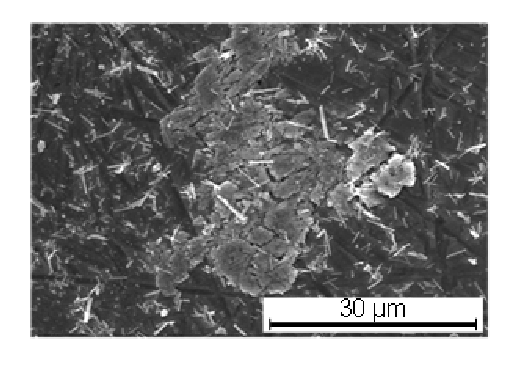
\includegraphics[scale=1.0]{slike/slika_mikroskop}
  \caption{Slika posneta z elektronskim mikroskopom \cite{bazant_1991}.} \label{fig:slika_mikroskop}
\end{centering}
\end{figure}

\begin{figure}[ht!]
\begin{centering}
  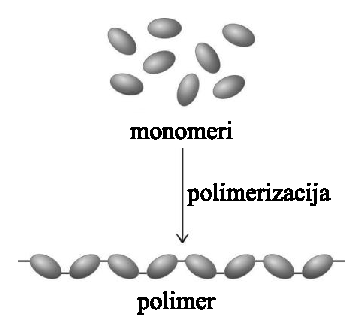
\includegraphics[scale=1.0]{slike/neke_molekule}
  \caption{Shematski prikaz postopka polimerizacije  \cite{Doe_1991, Bazant_2008}.} \label{fig:neke_molekule}
\end{centering}
\end{figure}

Naslov slike z zaporedno številko slike in kratkim opisom naj bo pod sliko, sredinsko poravnan glede na sliko in besedilo. Opis slike naj se začne z veliko začetnico in zaključi s končnim ločilom. Priporočljivo je, da so imena oz. opisi slik (kot tudi preglednic) kratki, saj je iz vidika kasnejše izdelave kazala slik (oz. preglednic) to bolj primerno.

Slike morajo biti berljive, jasne in pregledne. Slike morajo biti dobre kvalitete in v slovenskem jeziku. Če je na sliki diagram, morajo biti veličine in enote vseh osi jasno in dosledno označene. Na mikroskopskih posnetkih mora biti ustrezno označena dolžinska skala. Slike, ki so preslikane z optičnimi bralniki, naj bodo v čim boljši ločljivosti. Slike, ki jih ustvarjate sami s programi kot so CorelDraw, Photoshop, PowerPoint idr., naj bodo shranjene v formatu *.emf (ang. Enhanced Metafile) ali *.eps (ang. Encapsulated PostScript). Na ta način bodo pri pretvarjanju dokumenta v *.pdf obliko ohranjene vse podrobnosti na sliki in tudi pri tiskanju bo zagotovljena najvišja možna kvaliteta.
	
Vsaka slika (npr. tudi sliki \ref{fig:neke_molekule} in \ref{fig:2_grafa}) naj bo smiselno umeščena v besedilo. Običajno sliko umestimo pod odstavek, v katerem jo prvič omenimo. Če sliko zaradi bolj tekočega oblikovanja besedila umestimo drugače, naj bo vsekakor umeščena v bližini prve omembe v besedilu. Če sta sliki umeščeni ena pod drugo, naj bosta med naslovom prve slike in drugo sliko 2 prazni vrstici.

\begin{figure}
    \begin{subfigure}[b]{.45\linewidth}
        \centering 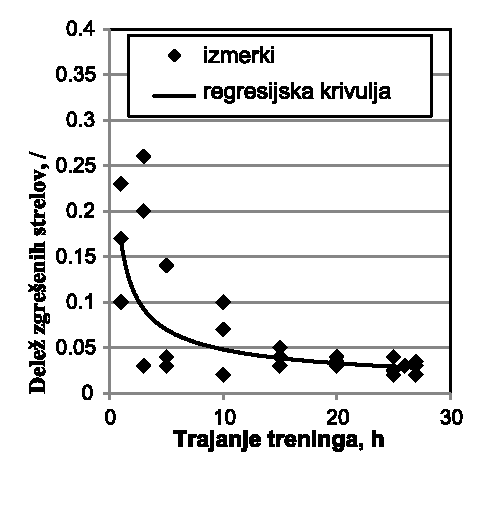
\includegraphics[scale=0.7]{slike/graf_1}
        \caption{}\label{subfig:graf1}
    \end{subfigure}%
    \quad
    \begin{subfigure}[b]{.45\linewidth}
        \centering 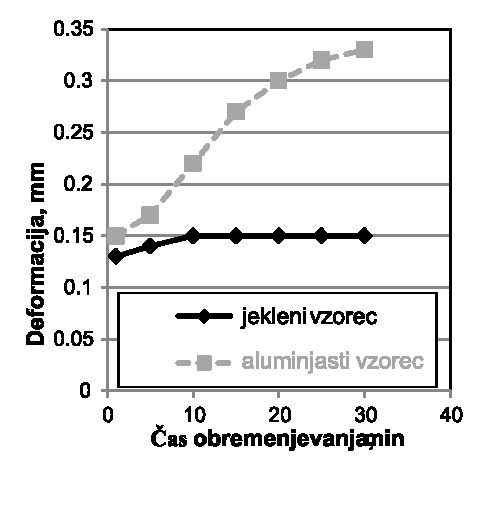
\includegraphics[scale=0.7]{slike/graf_2}
        \caption{}\label{subfig:graf2}
    \end{subfigure}

    \caption{(a) Odvisnost deleža zgrešenih strelov na tekmovanju v odvisnosti od časa treninga pred njim in (b) deformacija v odvisnosti od časa obremenjevanja za dva različna vzorca.}\label{fig:2_grafa}
\end{figure}

\begin{figure}[ht!]
\begin{centering}
  \includegraphics[scale=1.0]{slike/voda_in_nekej}
  \caption{Časovno sosledje padca projektila v vodo z višine (a) 2,1 m; in (b) 4,1 m \cite{Gonzalez_2014}.} \label{fig:voda_in_nekej}
\end{centering}
\end{figure}

Kot je prikazano na slikah \ref{fig:2_grafa} in \ref{fig:voda_in_nekej}, lahko več povezanih diagramov združite v eno sliko, pri čemer jih jasno ločite na podsklope, t.j. (a) in (b), pri tem pa pazite na preglednost.

Če je slika povzeta po določenem viru, je to potrebno citirati, kot je tudi prikazano na sliki \ref{fig:slika_mikroskop}. Tudi vse slike drugih avtorjev morajo biti citirane.

\section{Enačbe}\label{sec:enacbe}

Oblikovanje enačbe je v \LaTeX u avtomatsko. Pojasnilo enačbe mora biti v tekstu.
\begin{equation}\label{eqn:e}
e = m\,c^2
\end{equation}
\begin{equation}\label{eqn:e_cel}
e_{\text{cel}}=\sum_{i=1}^{n}\,m_{i}c^2
\end{equation}
\begin{equation}\label{eqn:Nu}
N_{\text{u}} = \frac{0{,}34}{Pr_{\text{L},i}\cdot 2{,}3A}
\end{equation}

V nadaljevanju teksta, če je to potrebno, se sklicuje na ustrezno številko enačbe, npr. na enačbo \eqref{eqn:e}.

Za oznake veličin in druge simbole običajno uporabljamo črke latinske in grške abecede, včasih z dodatki indeksov in drugih znakov. Kot je prikazano v enačbah \eqref{eqn:e_cel} in \eqref{eqn:Nu}, morajo biti simboli, torej oznake veličin, npr. $e$ ali $Pr$, pisane v kurzivnem (poševnem) tisku. Za simbolom ne postavljamo pike, razen če se s simbolom konča poved.

Indekse običajno uporabimo, kadar imata dve veličini enak simbol, ali pa če želimo veličino dodatno opredeliti (npr. $_{\text{max}}$ kot največji, $_{\text{cel}}$ kot celoten, $_{\text{z}}$ kot začetni ipd.). Indekse, ki označujejo fizikalne veličine, pišemo v kurzivnem (poševnem) tisku, opisni indeksi, ki služijo dodatnemu opredeljevanju veličin, npr. »cel« v $e_{\text{cel}}$ ali »L« v $Pr_{\text{L},i}$, pa morajo biti pisani v normalnem (pokončnem) tisku. Tudi indekse, ki so sestavljeni iz številk, pišemo v normalnem (pokončnem) tisku (npr. $A_1$), indekse iz črk, ki označujejo štetje oz. številke (npr. »i« v $m_i$ ali v $Pr_{\text{L},i}$) pa pišemo v kurzivnem (poševnem) tisku.

Za pravilno navajanje fizikalnih veličin, konstant, indeksov in ostalih elementov v enačbah upoštevajte »Priporočila avtorjem študijskih in strokovnih publikacij na Fakulteti za strojništvo v Ljubljani« avtorja viš.~pred.~dr.~Stropnika \cite{stropnik_1997}.

\section{Citiranje in navajanje virov}\label{sec:citiranje}

Pri citiranju upoštevajte pravila citiranja, ki ne veljajo le za zaključna dela, temveč tudi v splošnem za vsako predstavitev, v kateri sta uporabljeni intelektualna ali materialna lastnina drugih avtorjev. Kot vire v čim večji meri uporabljajte \textbf{novejšo relevantno mednarodno strokovno} literaturo. Spletni viri lahko predstavljajo \textbf{največ 25 \%} vseh virov, uporabljenih v zaključnem delu.

Vsa uporabljena literatura se v besedilu naloge navaja sproti po zaporednih številkah v \textbf{oglatem oklepaju}, zato naj bo tudi popis bibliografije oštevilčen v skladu z zaporedjem pojavljanja citatov v dokumentu. Primeri so prikazani v naslednjih povedih:
\begin{itemize}
\item V delu Bažanta in sodelavcev \cite{bazant_1991} je podan pregled vplivov na stabilnost konstrukcij.
\item V delu Bažanta et al. \cite{bazant_1991} je podan pregled vplivov na stabilnost konstrukcij.
\item Leta 2005 sta Bažant in Cedolin \cite{bazant_1991} predstavila uporabo modalne analize pri pre\-ra\-ču\-nu stabilnosti konstrukcij.
\end{itemize}

Zaporedna številka vira, na katerega se sklicujemo v oglatem oklepaju, se ponovi v popisu literature (glej \ref{sec:vzorci_lit} \nameref{sec:vzorci_lit}), pri kasnejšem ponovnem sklicevanju na isto referenco pa uporabimo enako številko kot pri prvem sklicu. Vse to je v \LaTeX u avtomatsko izvedeno, vendar končna kontrola vsekakor ni odveč.

Popis uporabljene literature naj bo levo poravnan (ang. align left) ter oblikovan v skladu s primeri v tej predlogi (glej poglavji \ref{sec:vzorci_lit} \nameref{sec:vzorci_lit} ter 7 Literatura) ter naj v splošnem obsega naslednje podatke:
\begin{itemize}
\item avtor, naslov dela, založba in kraj ter letnica izdaje, če gre za monografijo oz. \textbf{knjigo},
\item avtor, naslov poglavja, urednik, naslov knjige, založba, kraj in letnica izdaje ter številka začetne in zadnje strani poglavja, če gre za \textbf{poglavje v knjigi} oz. monografiji,
\item avtor, naslov članka, ime revije, številka revije, letnica izdaje ter številka začetne in zadnje strani članka, če gre za \textbf{članek} iz revije,
\item avtor, naslov prispevka, urednik ter naslov zbornika, kraj in datum konference (oz. objave zbornika) ter številka začetne in zadnje strani prispevka, če gre za \textbf{prispevek na konferenci},
\item avtor (če je naveden), naslov dela, spletni naslov, čas dostopa, če gre za vir iz \textbf{spletne strani},
\item avtor, naslov dela, tip dela, kraj in leto objave, če gre za \textbf{doktorsko disertacijo} ali drugo \textbf{zaključno delo}.
\end{itemize}

Ob sklicu na vir lahko pri več avtorjih namesto »in sodelavci« uporabimo »et al.«, na primer: V delu Bažanta et al. \cite{bazant_1991} je podan pregled vplivov\ldots

Vzorci popisa literature so podani v nadaljevanju. Z navedbo naštetih in (ali) drugih ustreznih podatkov pri virih, kot so na primer: referati s konferenc, patenti, standardi, predpisi, prospekti, elaborati, druge diplome, oz. pri navajanju literature upoštevajte še:
\begin{itemize}
\item SIST ISO 690: 1987(E) Documentation – Bibliographic references: Content, form and structure; ter
\item SIST ISO 690 – 2 : 1997(E) : Electronic documents or parts thereof.
\end{itemize}


\subsection{Vzorci popisa literature}\label{sec:vzorci_lit}

Za knjige:
\begin{itemize}
\item[{[1]}] Z.~P. Ba\v{z}ant, L.~Cedolin: \emph{Stability of Structures: Elastic,
  Inelastic, Fracture, and Damage Theories}. Oxford University Press, New York,
  1991.
\item[{[5]}] J.~Stropnik: \emph{Priporočila avtorjem študijskih in strokovnih publikacij
  na Fakulteti za strojništvo v Ljubljani}. Fakulteta za strojništvo,
  Ljubljana, 1997.
\end{itemize}

Za poglavja v knjigi:
\begin{itemize}
\item[{[2]}] J.~Doe: \emph{Earthquake stability}. V: Z.~P. Ba\v{z}ant, L.~Cedolin (ur.):
  \emph{Stability of Structures: Elastic, Inelastic, Fracture, and Damage
  Theories}. Oxford University Press, New York, 1991, str. 124--157.
\end{itemize}

Za revije:
\begin{itemize}
\item[{[3]}] Z.~P. Ba\v{z}ant, L.~Cedolin: \emph{Noise control}. Journal of Sound and
  Vibration \textbf{111}(2008) str. 42--50.
\item[{[4]}] J.~Gonzalez-Gutierrez, J.~L. Carillo-Estrada, J.~C. Ruiz-Suarez:
  \emph{Penetration of granular projectiles into a water target}. Scientific
  reports \textbf{4}:6762 (2014) str. 1--5.
\end{itemize}

Za konferenčne prispevke:
\begin{itemize}
\item[{[6]}] Z.~P. Ba\v{z}ant, L.~Cedolin: \emph{Modalna analiza}. V: B.~Podskrajnik (ur.):
  \emph{Kuhljevi dnevi: Zbornik referatov}. Ljubljana, Slovenija, 2005, str.
  2--5.
\item[{[7]}] Z.~P. Ba\v{z}ant, L.~Cedolin: \emph{Modal analysis}. V: S.~Smith (ur.):
  \emph{Proceedings of the 22. Congress of Polymers}. London, UK, 2007, str.
  3--8.
\end{itemize}

Za spletne vire z znanim avtorjem:
\begin{itemize}
\item[{[8]}] C.~Kogoj: \emph{Modalna analiza: izbrana poglavja iz {DTD}}. Dostopno na:
  \url{http://lab.fs.uni-lj.si/ldtd/Gradivo_za_studente/DTD/Pregled\%20teorije.pdf},\\
  Ogled: 11. 1. 2012.
\end{itemize}

Za publikacije organizacij (tiskane ali objavljene na spletnih straneh):
\begin{itemize}
\item[{[9]}] {Merkur d.d.}: \emph{Letno poročilo podjetja Merkur d.d. Kranj}, 2005.
\item[{[10]}] {Statistični urad republike Slovenije}: \emph{Statistični letopis Republike
  Slovenije 2009}. Statistični urad republike Slovenije, Ljubljana, 2009.
\item[{[11]}] {Statistični urad republike Slovenije}: \emph{Standardna klasifikacija
  dejavnosti 2005}. Dostopno na:
  \url{http://www.stat.si/klas/tabela.aspx?cvn=1895}, Ogled: 10. 1. 2012.
\end{itemize}

Za spletne strani organizacij, društev, posameznikov:
\begin{itemize}
\item[{[12]}] \emph{M Kariera – Zaposlitveni portal}. Dostopno na:
  \url{http://www.mercator.si/kariera}, Ogled: 10. 1. 2012.
\end{itemize}

Za spletne baze, enciklopedije, slovarje ipd.:
\begin{itemize}
\item[{[13]}] \emph{Engineering}. V Encyclopedia Britannica online. Dostopno na:
  \url{http://student.britannica.com/comptons/article-9274119/engineering},
  Ogled: 8. 1. 2012.
\item[{[14]}] \emph{Poslovna aplikacija}. V eSlovarju. Dostopno na:

  \url{http://www.eslovar.com/besedilo.asp?id=1563}, Ogled: 8. 1. 2012.
\end{itemize}

Za zakonodajo (uradni listi, pravilniki, standardi):
\begin{itemize}
\item[{[15]}] \emph{Zakon o gospodarskih družbah}, {U}radni list RS št. 42/2006, 60/2006
  popr., 26/2007-ZSDU-B, 33/2007-ZSReg-B, 67/2007-ZTFI (100/2007 popr.),
  10/2008, 68/2008, 23/ 2009; Odl. US: U-I-268/06-35.
\item[{[16]}] \emph{Zakon o okoljskih predpisih}, {U}radni list RS št. 72/2009-UPB2,
  65/2010.
\item[{[17]}] {ISO 2573:1977}: \emph{Tensile testing systems – Determination of K-value}.
\item[{[18]}] {DIN 4768:1990}: \emph{Determination of surface roughness values R$_a$, R$_z$,
  R$_{max}$}.
\item[{[19]}] {JIS B 0601:2001}: \emph{Geometrical product specifications (GPS) profile
  method – Terms, definitions and surface texture parameters}.
\end{itemize}

Za doktorske disertacije in druga zaključna dela:
\begin{itemize}
\item[{[20]}] A.~Novak: \emph{Izdelava avtomatiziranega stroja za lupljenje krompirja}:
  \emph{Doktorska disertacija}, Univerza v Ljubljani, 2015.
\end{itemize}

Popis literature je v \LaTeX u izveden avtomatsko, glede na vašo bazo bibliografij (ki se v primeru predloge nahaja na References.bib) ter izbrane makre, ki ustrezno generirajo \TeX~sintakso bibliografije. Za zaključna dela na Fakulteti za Strojništvo je izdelan ustrezen makro, ki se nahaja v fs\_zakljucne\_naloge.bst. Uporabo le-tega definirate z ukazom \verb|\bibliographystyle{fs_zakljucne_naloge}| v glavni datoteki.

Sklici na popis literaturo so avtomatsko generirani, npr: \cite{bazant_1991}, \cite{Doe_1991},  \cite{Bazant_2008}, \cite{Gonzalez_2014, Bazant_2005} \cite{Bazant_2007, Kogoj_DTD, Merkur_2005, SURS_2009, SURS_2005, MKariera, Encyclopedia, Posl_app, ZGD, ZOP}, \cite{ISO_2573}, \cite{DIN_4768}, \cite{DIN_4768} in \cite{JISB0601, Novak_2015}.





